\chapter{Asistente web interactivo para la simplificación de textos a Lectura Fácil}
\label{cap:asistenteWeb}


\chapterquote{La tecnología hace posible lo que antes era imposible. El diseño hace que sea real}{Michael Gagliano}

En este capítulo se describirán los requisitos necesarios que debe cumplir nuestro asistente para un correcto funcionamiento. Además mostraremos un recorrido por las diferentes vistas que encontrará el usuario editor durante el uso del mismo.



\section{Requisitos del asistente web interactivo para la simplificación de textos}\label{sec:requisitosAplicacion}

Para ayudar a los distintos destinatarios descritos en el capítulo \ref{cap:estadoDeLaCuestion}, sección \ref{subsec:gruposLectores}, uno de los primeros pasos ha sido valorar qué funcionalidades era necesario tener definidas antes del desarrollo del asistente. Éste deberá servir de apoyo al editor al realizar una serie de operaciones sobre un texto, artículo, relato, etc. para facilitar la adaptación del mismo a Lectura Fácil. 

Hay que tener en cuenta que la tarea de adaptación de textos puede ser costosa y tediosa en muchas ocasiones. Para evitarlo, gracias a este asistente, el usuario tendrá a su alcance funcionalidades que tienen como objetivo una simplificación y mejor comprensión del texto, teniendo, además, la posibilidad de realizar modificaciones manuales.

Tal y como se hizo referencia en el capítulo \ref{cap:estadoDeLaCuestion} (ver sección \ref{subsec:tareas}), es imprescindible poder hacer transformaciones y modificaciones en nuestro texto para poder hacerlo más accesible a un determinado público. Así pues, el asistente permite realizar una serie de operaciones que facilitará la adaptación de cualquier texto a LF permitiendo al usuario en todo momento realizar los ajustes manuales necesarios. Estas operaciones son las siguientes:

\begin{itemize}
	
	\item Hacer un resumen del texto introducido, favoreciendo una simplificación y eliminación de información redundante o poco relevante.
	\item  Detección de palabras que puedan ser más complejas de cara al lector.
	\item Facilitar el reemplazo de palabras por sinónimos que puedan ser más sencillos y accesibles al lector derivando en una simplificación léxica.
	\item Posibilidad de eliminar palabras, suprimiendo información no esencial que al lector no le aporte valor en la lectura.
	\item Permitir al editor añadir definiciones de términos que pueden ser añadidas como parte del texto final, aportando al lector información adicional sobre aquello que puede no serle familiar.
	\item  Intercambio sintáctico de una o varias palabras de orden de manera que el editor pueda colocarlas en favor de una mejor comprensión por parte del lector.
\end{itemize}

 

Una vez definidas las funcionalidades necesarias que incluye nuestro asistente, veremos en las siguientes secciones el flujo de trabajo que realizará el editor, donde se describirán las funcionalidades ya mencionadas anteriormente.





\section{Introducción de texto y selección de frases}
\label{introduccionTextoYFrases}
 El usuario editor debe de navegar a la dirección. \url{https://holstein.fdi.ucm.es/tfg/2021/simpli/} oara comenzar a adaptar su texto.
 La primera pantalla que visualizará el usuario editor será como la que muestra la Figura \ref{fig:interfazInicial}. En la parte superior de la pantalla encontrará una barra de navegación mientras que en la parte central de la misma se muestra el título del asistente, una descripción y un botón (\textbf{Introducir texto}). 
  \begin{figure}[h!]
 	\centering
 	
 	
 	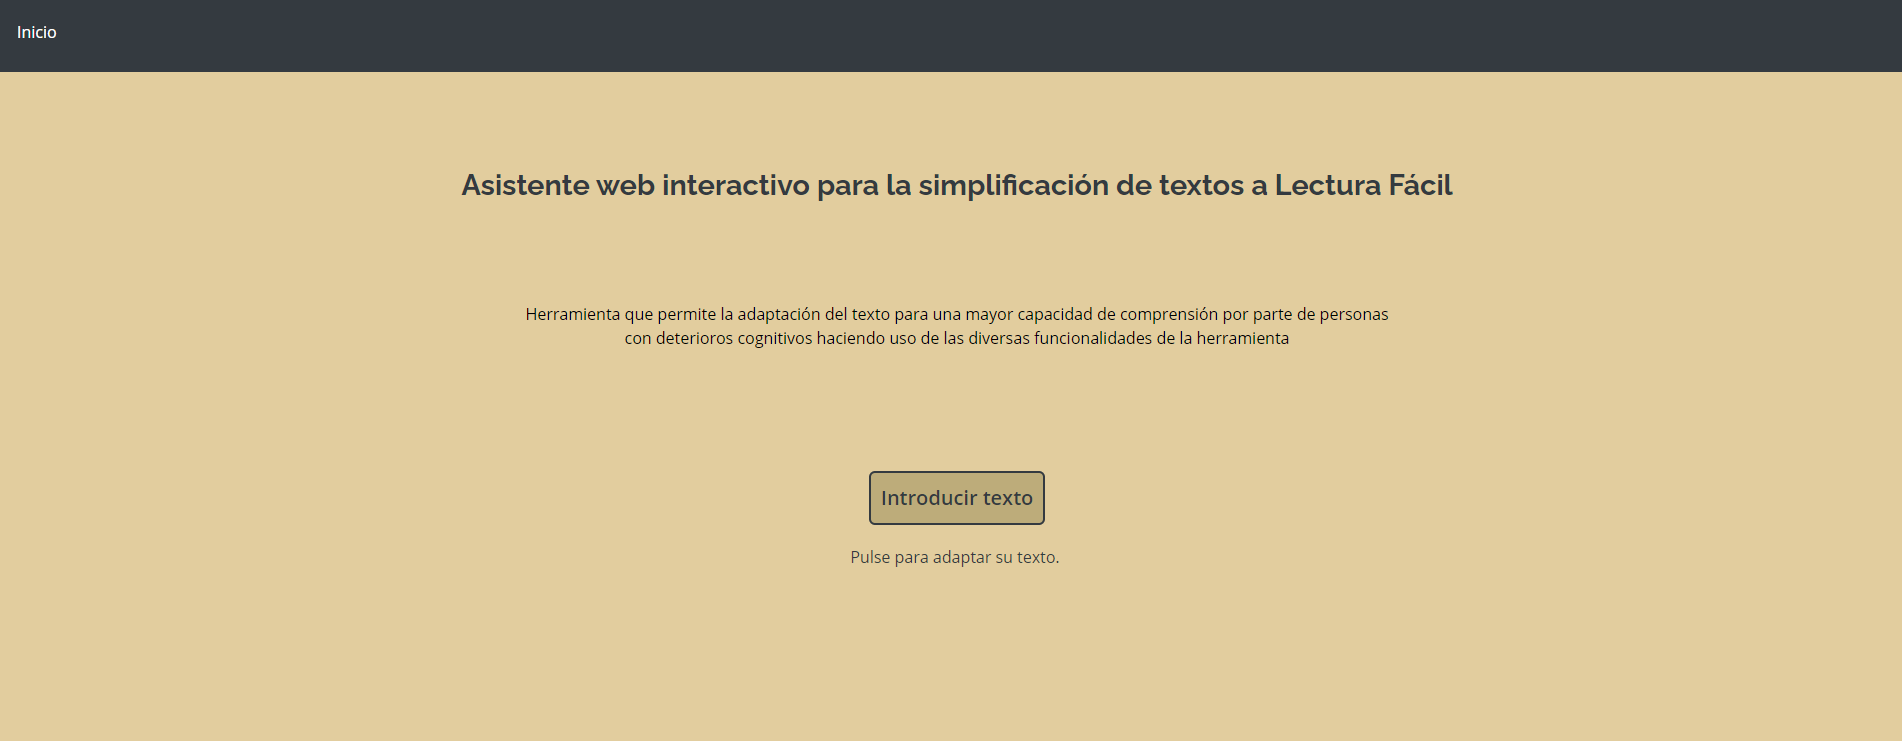
\includegraphics[scale=1]{Imagenes/Figuras/InterfazInicial}
 	
 	
 	\caption{Interfaz inicial del asistente.}
 	\label{fig:interfazInicial}
 \end{figure}
 
 Al pulsar en dicho botón se mostrará un panel lateral con las siguientes opciones:
 
 \begin{itemize}
 	\item \textbf{Texto original}: un  panel donde se introducirá el texto que queremos adaptar (ver Figura \ref{fig:interfazIntroduccionTexto}).
 	\begin{figure}[h!]
 		\centering
 		
 		
 		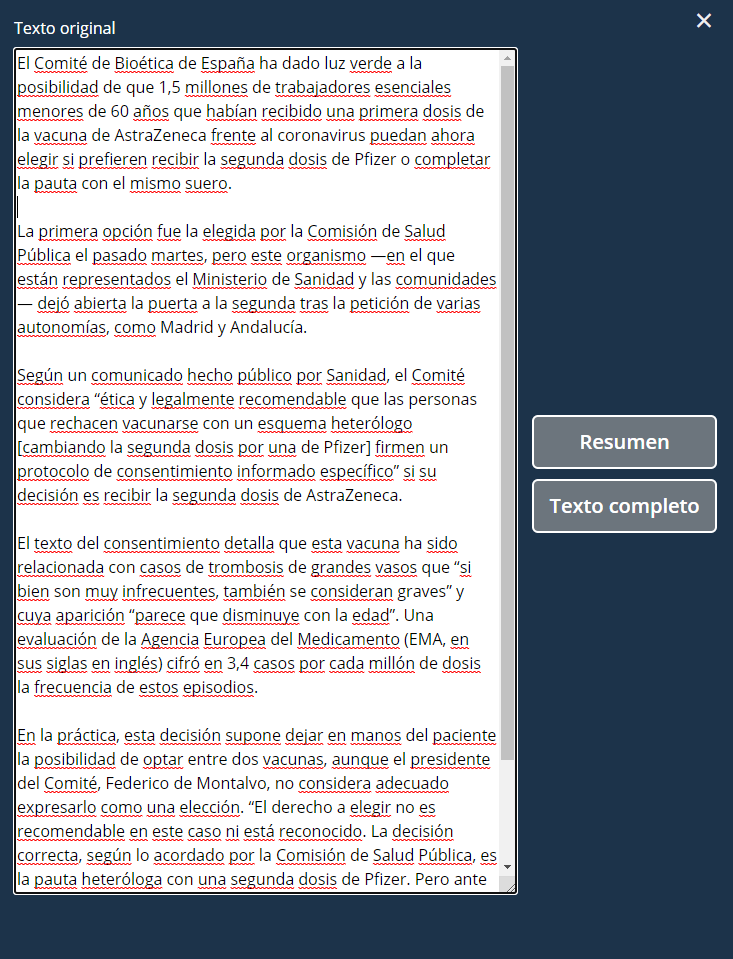
\includegraphics[scale=0.7]{Imagenes/Figuras/PanelIzquierdo}
 		
 		
 		\caption{Panel lateral de introducción de texto.}
 		\label{fig:interfazIntroduccionTexto}
 	\end{figure}
 	 	\item \textbf{Botón Resumen}: si pulsamos esta opción se mostrará una vista con una serie de frases resultado del resumen del texto original previamente introducido (véase Figura \ref{fig:interfazFraseTextoResumido}). Este botón permanecerá inactivo hasta que se introduzca texto. 
 	 	 	\item \textbf{Botón Texto completo}: si, por el contrario, pulsamos esta opción se mostrará el texto completo dividido en frases, también seleccionables (Figura \ref{fig:interfazIntroducirCompleto}). Al igual que el anterior botón también permanecerá inactivo hasta que el usuario introduzca texto. 
 	 	 \begin{figure}[h!]
 	 	 	\centering
 	 	 	
 	 	 	
 	 	 	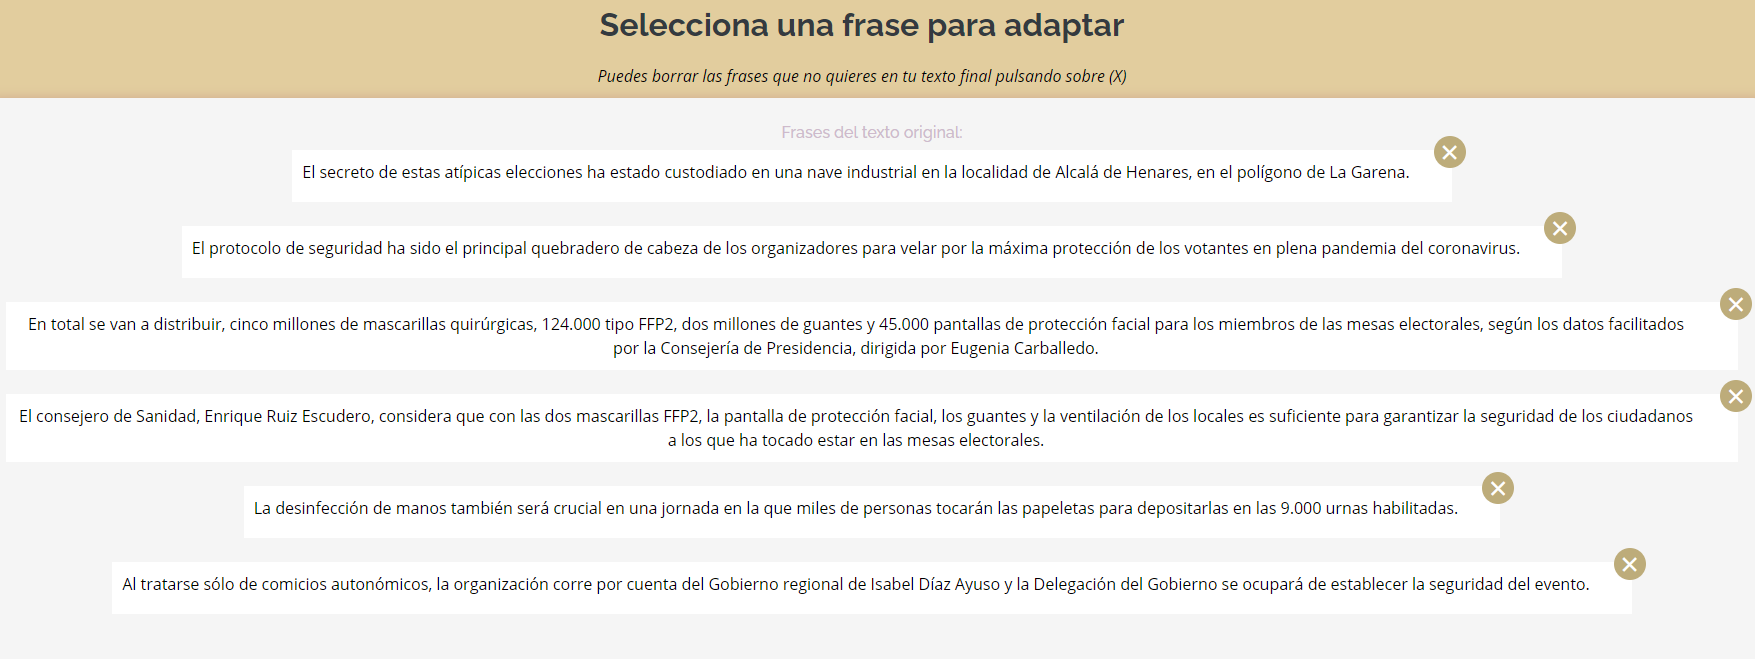
\includegraphics[scale=0.7]{Imagenes/Figuras/Resumen}
 	 	 	
 	 	 	
 	 	 	\caption{Frases partiendo del resumen.}
 	 	 	\label{fig:interfazFraseTextoResumido}
 	 	 \end{figure}
 	 	 
 	 	 
 	 	 \begin{figure}[h!]
 	 	 	\centering
 	 	 	
 	 	 	
 	 	 	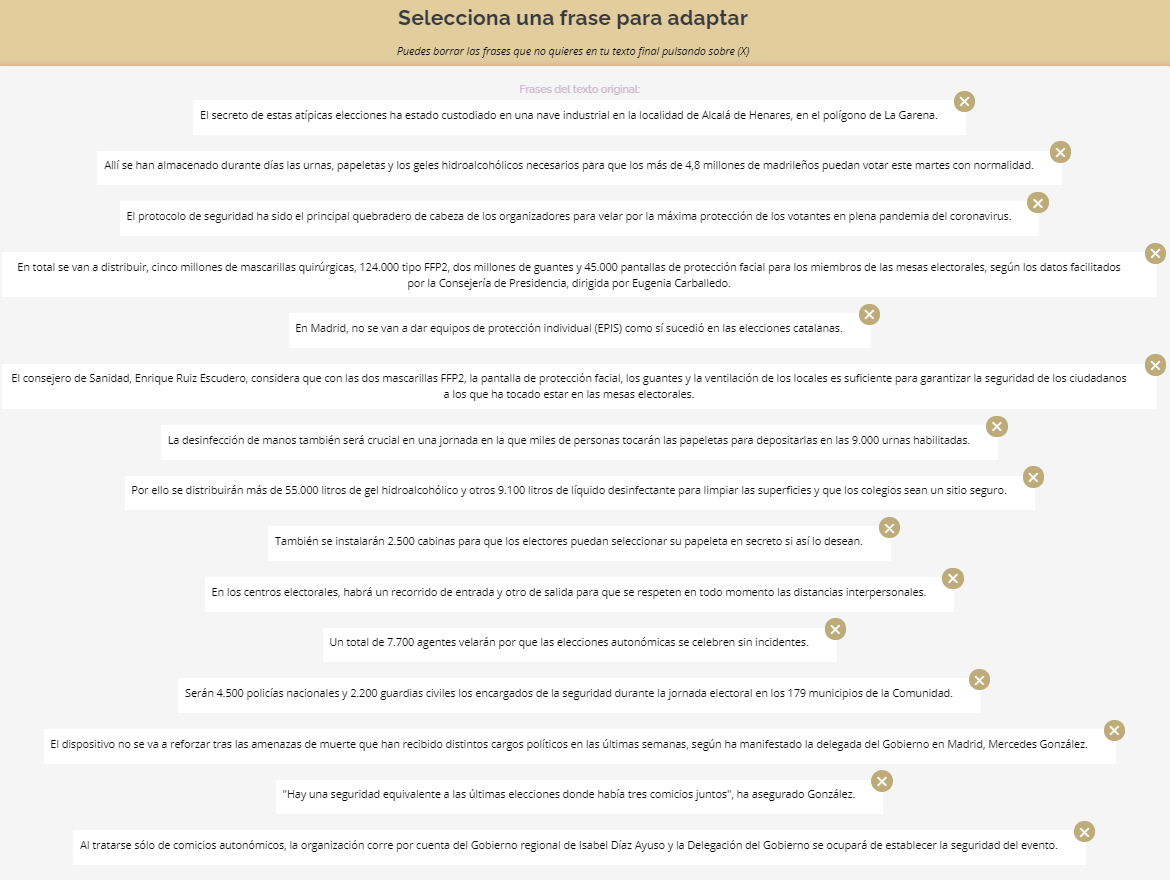
\includegraphics[scale=0.7]{Imagenes/Figuras/TextoCompleto}
 	 	 	
 	 	 	
 	 	 	\caption{Frases partiendo del texto completo.}
 	 	 	\label{fig:interfazIntroducirCompleto}
 	 	 \end{figure}	
 \end{itemize}

	Recordemos que en la Figura \ref{fig:interfazInicial} sólo contábamos con la pestaña de ``Inicio'' en la barra de navegación, la cual cambia añadiendo una nueva pestaña \textbf{``Texto original''}. Esta pestaña nos permitirá consultar siempre el texto original que hemos introducido y cambiar en cualquier punto del flujo la opción elegida detallada anteriormente (resumen o texto completo). 


\section{Adaptaciones sobre frases}

Al clicar sobre una frase como las que se muestran en las Figuras \ref{fig:interfazFraseTextoResumido} y \ref{fig:interfazIntroducirCompleto}, se cambiará a una vista donde aparecerá un árbol de dependencias (véase Figura \ref{fig:arbolDependencias}), que describe la estructura sintáctica de dicha frase, y que le servirá al usuario editor a la hora de adaptarla de una manera interactiva. 

En dicho árbol encontramos las unidades léxicas separadas de la frase, las cuales podremos pulsar y aplicar sobre ellas una serie de operaciones que se encuentran como botones en la parte inferior izquierda. Junto a estos, aparece una breve explicación de la funcionalidad (ver operaciones que podemos efectuar en la Figura \ref{fig:botonesFuncionales}) que detallaremos en el capítulo \ref{cap:implementacion}, sección \ref{subsec:implementacionAplicacionWeb}. 

En la parte superior de la pantalla el editor podrá visualizar en todo momento la frase previamente elegida y un enlace (\textbf{Volver a las frases}) para volver al listado de frases, en el caso de que se quiera elegir otra o retomar alguna que ya haya sido modificada.

 En la parte inferior derecha de la vista, tenemos el borrador del texto final (Ver Figura \ref{fig:borradorTextoFinal}) donde se puede visualizar la transformación de la frase seleccionada (en negrita) habiendo realizado, o no, las diferentes operaciones. 
\begin{figure}[h!]
	\centering	
	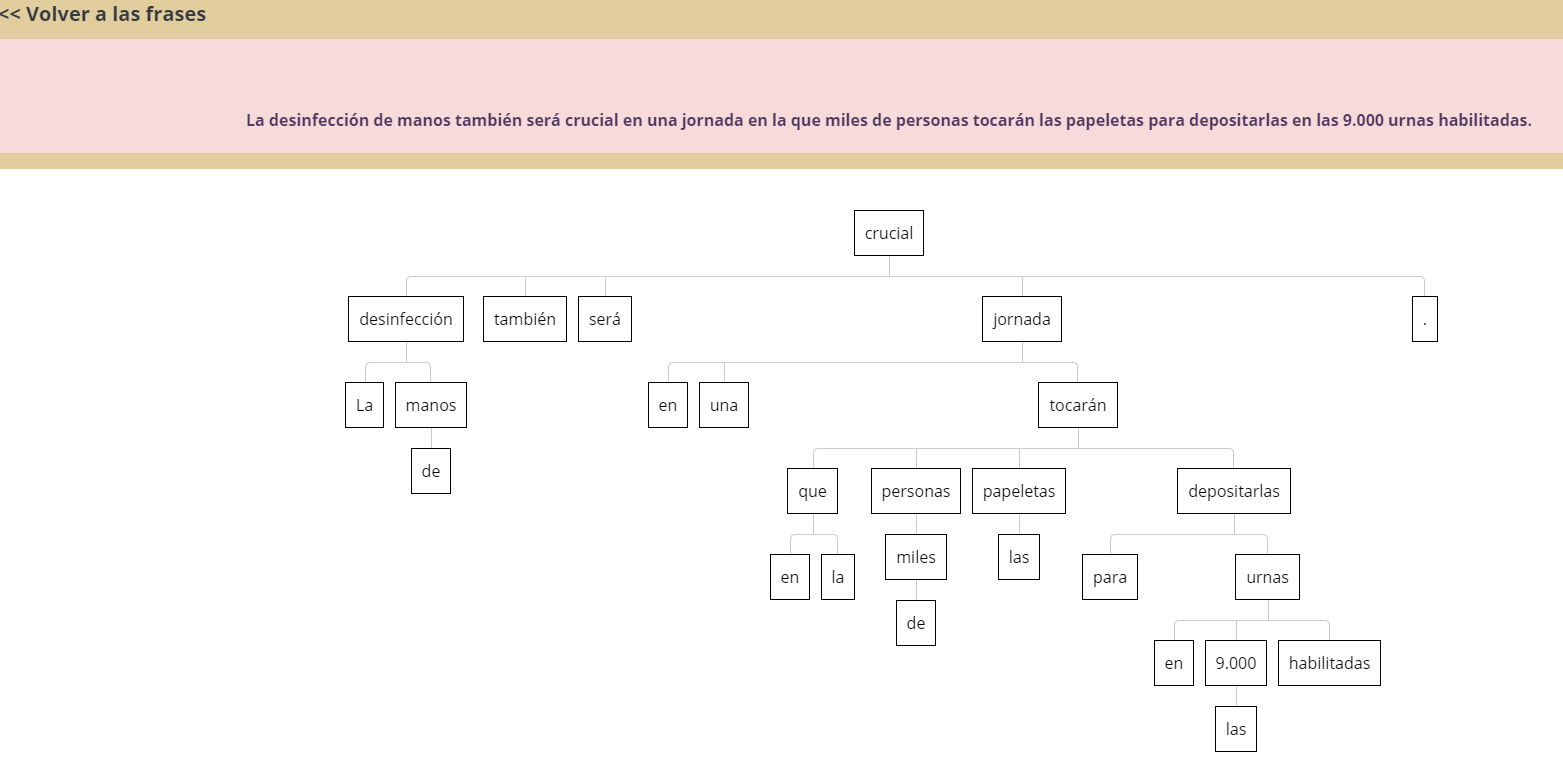
\includegraphics[scale=0.6]{Imagenes/Figuras/arbol}	
	\caption{Árbol de dependencias.}
	\label{fig:arbolDependencias}
\end{figure}
\begin{figure}[h!]
	\centering
	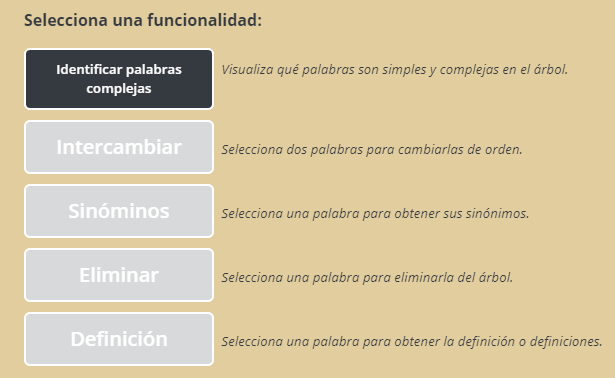
\includegraphics[scale=1.0]{Imagenes/Figuras/botonesFuncionales}
		\caption{Operaciones que podemos efectuar sobre los elementos del árbol de dependencias}
	\label{fig:botonesFuncionales}
\end{figure}
\begin{figure}[h!]
	\centering
	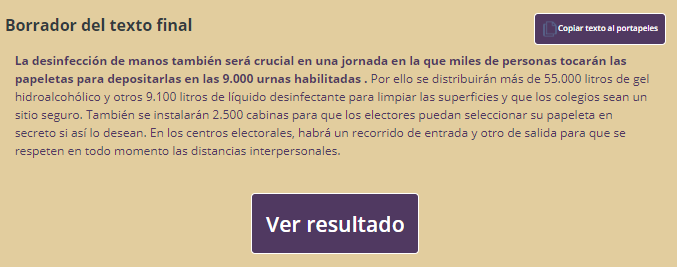
\includegraphics[scale=1.0]{Imagenes/Figuras/borradorTextoFinal}
	\caption{Borrador del texto final.}
	\label{fig:borradorTextoFinal}
\end{figure}


A continuación, describiremos en qué consisten, en qué situaciones y cómo el usuario debe utilizar cada una de las operaciones que se pueden efectuar.

\subsection{Palabras complejas}
Esta funcionalidad es de utilidad cuando el usuario editor desee conocer aquellos términos de la frase que pueden ser susceptibles de ser reemplazados por sinónimos que sean más asequibles de comprender para el lector o explicados en más detalle. El elemento visual que se encargará de esta función es el botón \textbf{Identificar palabras complejas}.

Una vez hagamos clic en este botón nuestro árbol de dependencias mostrará las palabras complejas. Como podemos ver en la Figura \ref{fig:palabrasComplejas}, aparece una leyenda en la parte superior izquierda del árbol, indicando el color en el que se colorean. Una vez pulsado, el texto del botón cambiará a \textbf{Desactivar palabras complejas} para poder volver a la vista original del árbol de dependencias. 
	 \begin{figure}[h!]
	\centering
	
	
	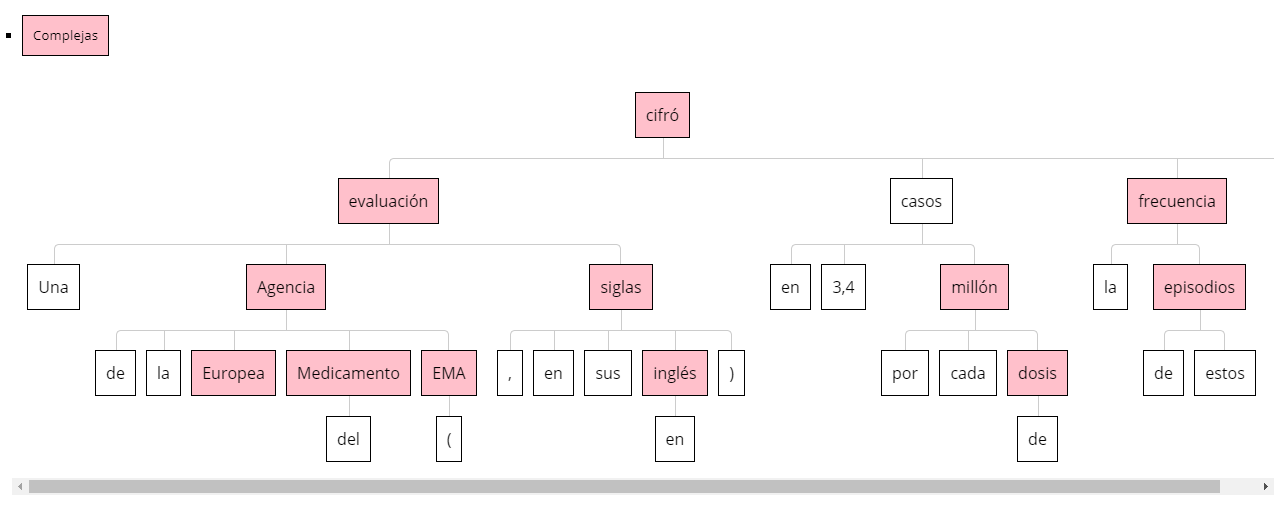
\includegraphics[scale=0.6]{Imagenes/Figuras/palabrasComplejas}
	
	
	\caption{Palabras complejas resaltadas en el árbol.}
	\label{fig:palabrasComplejas}
\end{figure}
\subsection{Intercambio de partes en el árbol de dependencias}
Puede ocurrir que el usuario editor desee modificar el orden sintáctico de la frase. Por ejemplo, se puede dar la situación de que la segunda parte de una frase sea más importante y por ende se quiera que el lector ponga más atención a esa parte poniéndola al principio. 

Para que esta funcionalidad se active es necesario tener seleccionadas dos palabras del árbol. Ambas palabras cambiarán de orden incluyendo también aquellas que dependan de las mismas. Se puede ver un ejemplo del intercambio de dos palabras en el árbol de dependencias en las figuras \ref{fig:eleccionIntercambio} y \ref{fig:intercambio}). El texto resultante quedaría como se muestra en la Figura \ref{fig:borradorIntercambio}. En cualquier momento, el usuario puede editar el texto para solucionar la concordancia minúsculas/mayúsculas en el caso de que sea necesario.


\begin{figure}[h!]
	\centering
	
	
	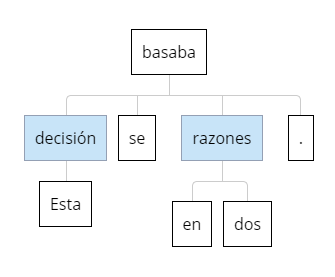
\includegraphics[scale=1]{Imagenes/Figuras/EleccionIntercambio}
	
	
	\caption{Elección de dos palabras para el intercambio.}
	\label{fig:eleccionIntercambio}
\end{figure}
\begin{figure}[h!]
	\centering
	
	
	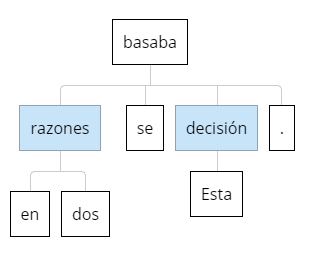
\includegraphics[scale=1]{Imagenes/Figuras/IntercambioArbol}
	
	
	\caption{Árbol de dependencias después del intercambio.}
	\label{fig:intercambio}
\end{figure}
\begin{figure}[h!]
	\centering
	
	
	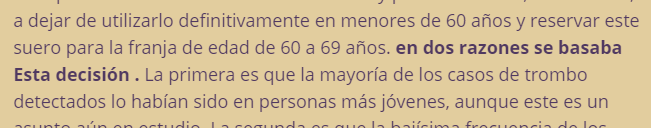
\includegraphics[scale=1]{Imagenes/Figuras/BorradorIntercambio}
	
	
	\caption{Resultado en el borrador del texto final tras el intercambio.}
	\label{fig:borradorIntercambio}
\end{figure}
\subsection{Sinónimos}
En ocasiones el usuario se verá en la necesidad de realizar una simplificación léxica sustituyendo una palabra por un sinónimo más conocido. Podrá hacer uso de ella pulsando sobre el botón (\textbf{Sinónimos}), siempre y cuando se haya seleccionado una palabra del árbol previamente. Una vez pulsado, se muestran, si existen, todos los sinónimos de la palabra elegida. En caso de que la palabra no tenga sinónimos aparecerá un texto informando de que carece de ellos. Si los tiene, se mostrará un listado de estos indicando cuáles son sencillos y cuáles no (ver opción sinónimos en la Figura \ref{fig:listaSinonimos}). En esta figura mostramos, por ejemplo, los sinónimos complejos y sencillos de la palabra ``dosis''.

	 \begin{figure}[h!]
	\centering
	
	
	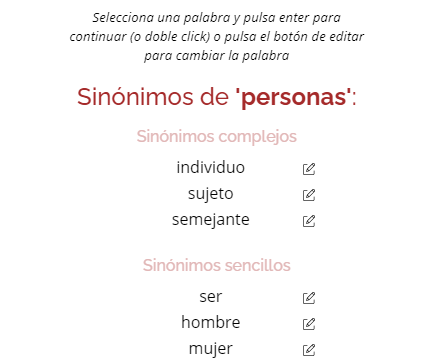
\includegraphics[scale=1.0]{Imagenes/Figuras/SinonimoPersona}
	
	
	\caption{Lista de sinónimos de una palabra seleccionada}
	\label{fig:listaSinonimos}
\end{figure}

 Llegados a este punto, se podrá seleccionar uno de ellos o bien haciendo doble clic o bien editándolo si fuese necesario para un significado coherente con la frase (concordancia en género, número, persona y conjugación), y posteriormente pulsar ``Enter'' para el cambio (véase la Figura \ref{fig:edicionSinonimos}). Aquí se edita el sinónimo sencillo ``parte'' por ``partes'', ya que por el contexto de la frase es conveniente adaptarlo a plural.


\begin{figure}[h!]
\centering


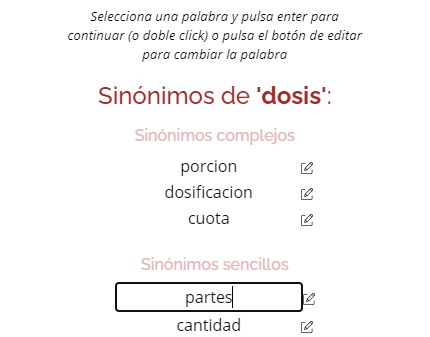
\includegraphics[scale=1.0]{Imagenes/Figuras/EditarSinonimo}


\caption{Interfaz de edición de sinónimos}
\label{fig:edicionSinonimos}
\end{figure}
Al hacer doble clic o ``Enter'', si lo hemos editado, se mostrará una ventana de diálogo (Aceptar y Cancelar) para asegurar si es realmente la acción que queremos realizar (ver Figura \ref{fig:modalSinonimos}). En el caso de que se elija ``Aceptar'', tanto en el árbol de dependencias como en el borrador del texto final se reemplazará la palabra (Figura \ref{fig:resultadoSinonimos}). En caso contrario, no habrá modificación alguna.

\begin{figure}[h!]
	\centering
	
	
	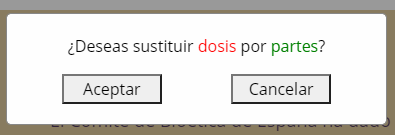
\includegraphics[scale=1.0]{Imagenes/Figuras/modalSinonimos}
	
	
	\caption{Ventana de diálogo de reemplazo de sinónimo.}
	\label{fig:modalSinonimos}
\end{figure}

\begin{figure}[h!]
	\centering
	
	
	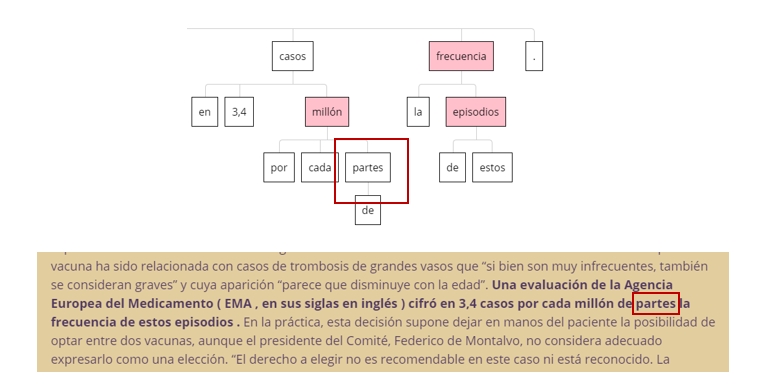
\includegraphics[scale=1.0]{Imagenes/Figuras/CambioSinonimoArbolBorrador}
	
	
	\caption{Resultado de reemplazo del sinónimo tanto en el árbol de dependencias como en el borrador}
	\label{fig:resultadoSinonimos}
\end{figure}
\subsection{Eliminar partes en el árbol de dependencias}

El usuario editor puede encontrarse con frases que no requieren de ciertas palabras para que se capte la esencia de las mismas por parte del lector. Es por ello por lo que tiene la opción de eliminar términos a su disposición. Es necesario seleccionar una palabra del árbol para que esta funcionalidad pueda llevarse a cabo y se suprimen tanto a la palabra como aquellas que dependan de la misma. En las Figuras \ref{fig:eliminacionPrevia} y \ref{fig:eliminacion} vemos la palabra seleccionada, en este caso ``acordado'', que queremos eliminar, y el resultado de su eliminación en el árbol y en el texto del borrador final.
	 \begin{figure}[h!]
	\centering
	
	
	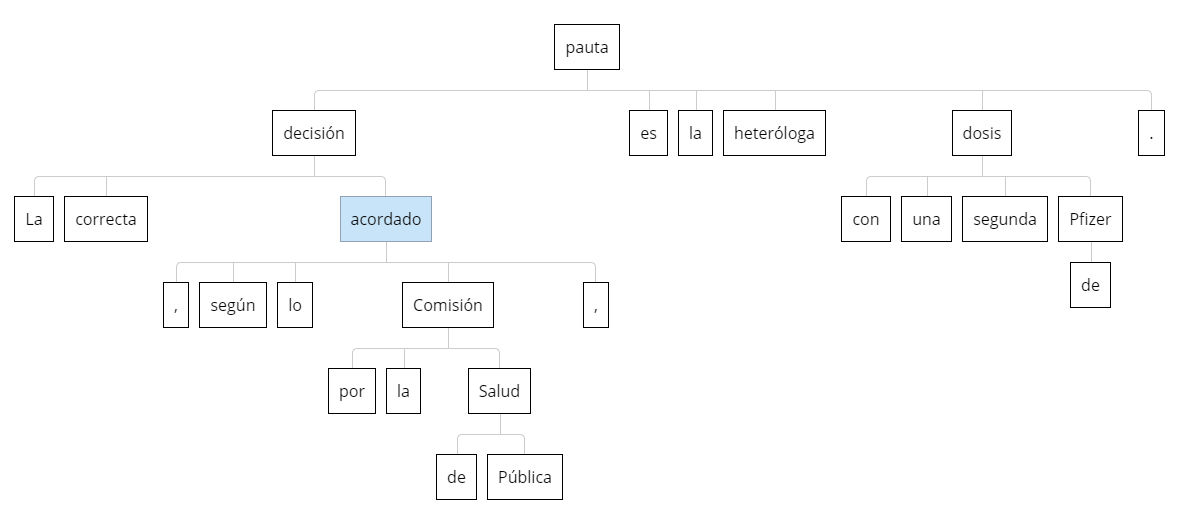
\includegraphics[scale=0.6]{Imagenes/Figuras/EleccionEliminacion}
	
	
	\caption{Árbol antes la eliminación de una palabra.}
	\label{fig:eliminacionPrevia}
\end{figure} 
	 \begin{figure}[h!]
	\centering
	
	
	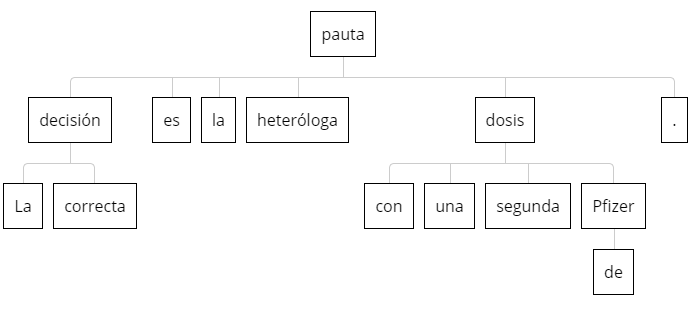
\includegraphics[scale=0.9]{Imagenes/Figuras/EliminacionSubarbol}
	
	
	\caption{Árbol tras la eliminación de una palabra.}
	\label{fig:eliminacion}
\end{figure} 
El resultado de la frase modificada lo podemos ver en la Figura \ref{fig:resultadoEliminar}.
	 \begin{figure}[h!]
	\centering
	
	
	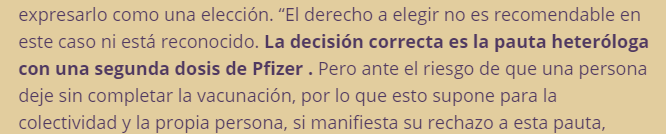
\includegraphics[scale=1]{Imagenes/Figuras/BorradorEliminacion}
	
	
	\caption{Borrador del texto final tras la eliminación de una palabra.}
	\label{fig:resultadoEliminar}
\end{figure} 

\subsection{Definiciones respecto a una palabra}
 Gracias a esta funcionalidad, el encargado de adaptar texto podrá nutrir el texto final con definiciones de uno o varios términos que considere que puedan precisar de alguna aclaración. 
 
 Seleccionando una palabra en el árbol, el botón (\textbf{Definición}) se activará. Al pulsar sobre este se mostrará un listado con todas las acepciones, si las tiene, de la palabra seleccionada. Vemos, por ejemplo, las de la palabra ``correcta'' en la Figura \ref{fig:definiciones}. Haciendo clic en una de ellas, ésta se adjuntará a modo de glosario como parte del texto final, sirviendo de apoyo a la comprensión del mismo (ver Figura \ref{fig:definicionesBorrador}). En caso de que no posea definiciones (por ejemplo, nombres propios) aparecerá un texto informando que carece de ellas.
 	 \begin{figure}[h!]
 	\centering
 	
 	
 	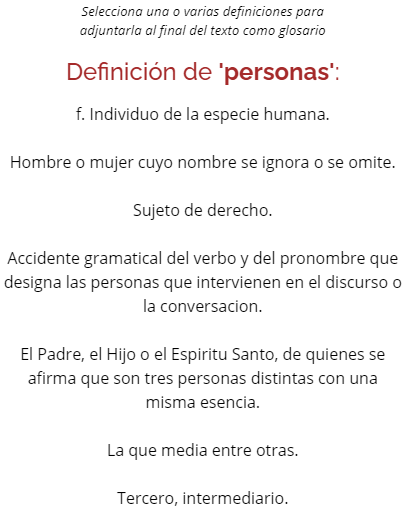
\includegraphics[scale=0.8]{Imagenes/Figuras/DefinicionesPersonas}
 	
 	
 	\caption{Listado de las definiciones}
 	\label{fig:definiciones}
 \end{figure}
 	 \begin{figure}[h!]
	\centering
	
	
	\includegraphics[scale=0.8]{Imagenes/Figuras/GlosarioBorrador}
	
	
	\caption{Glosario adjunto al borrador del texto final.}
	\label{fig:definicionesBorrador}
\end{figure}
\subsection{Resultado de la adaptación}
 
Cuando hayamos considerado que el texto esté adaptado a nuestras necesidades, podemos visualizarlo haciendo clic en el botón (\textbf{Ver resultado}), el cuál lo encontramos en la parte inferior derecha del borrador del texto final (ver Figura \ref{fig:botonResultado}). Al pulsarlo, se desplegará un panel editable en la parte derecha con el mismo texto que obtuvimos en el borrador (este panel lo podemos ver en la Figura \ref{fig:panelFinal}). Esto es útil, por ejemplo, si el editor desea incluir la acepción dentro del contexto del texto final 
\begin{figure}[h!]
	\centering
	
	
	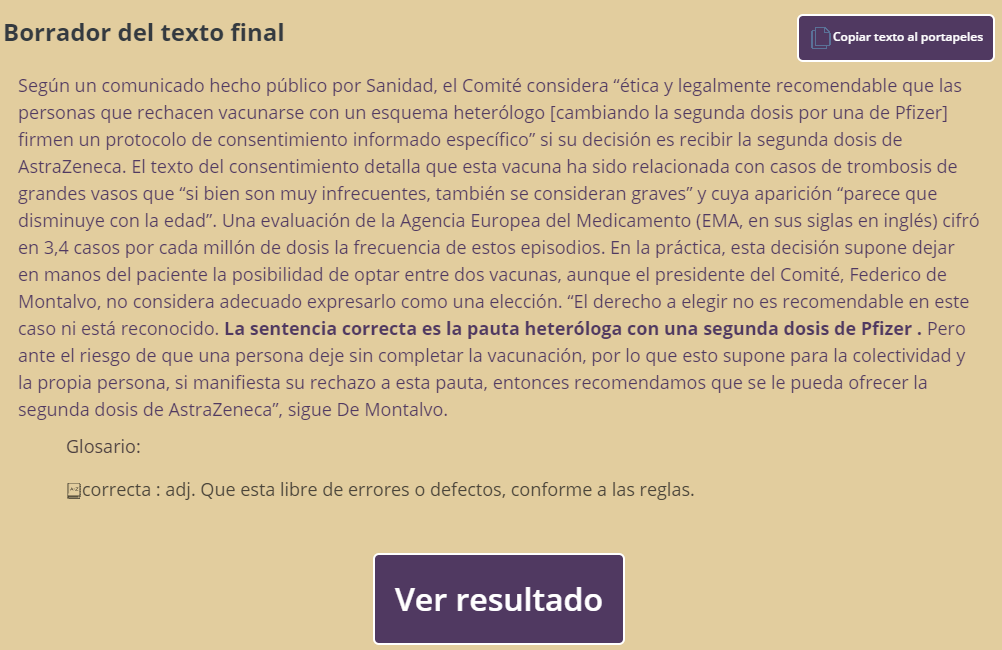
\includegraphics[scale=0.8]{Imagenes/Figuras/verResultado}
	
	
	\caption{Botón Ver resultado junto al borrador del texto final.}
	\label{fig:botonResultado}
\end{figure}
\begin{figure}[h!]
	\centering
	
	
	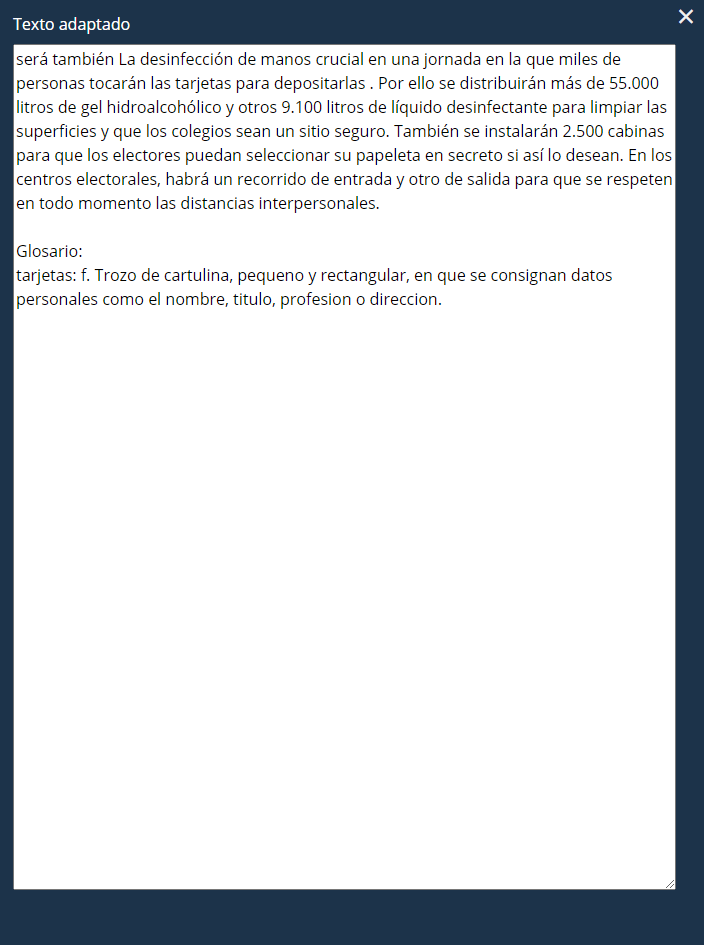
\includegraphics[scale=0.8]{Imagenes/Figuras/PanelDerecho}
	
	
	\caption{Panel con el resultado final del texto adaptado}
	\label{fig:panelFinal}
\end{figure}

Como hemos visto en la Figura \ref{fig:botonResultado}, también contamos con un botón \textbf{Copiar al portapapeles} que nos da la opción de copiar el texto del borrador para poder introducirlo en cualquier herramienta externa más fácilmente.


